\chapter{Umsetzung}
\label{chapter:implementation}
    In diesem Kapitel wird die Umsetzung des System erläutert.
    Zunächst wird die zur Implementierung verwendete Software näher erläutert.
    Anschließend werden Front- und Backend kurz vorgestellt und mit dem Entwurf aus Kapitel \ref{chapter:design} verglichen.
    Zur Versionsverwaltung der verwendeten Komponenten wurde die GitHub Organisation BwolfJena\footnote{\href{https://github.com/BWolfJena}{https://github.com/BWolfJena}} erstellt.
    
    \section{Verwendete Software}

        Für die lokale Entwicklung wurde als Basis \textit{Laradock}\footnote{\href{http://laradock.io/}{http://laradock.io/}} verwendet und auf die benötigte Software angepasst.
        Diese modifizierte \textit{Laradock} Variante wurde als \textit{git submodule} in das Hauptrepository \textit{BWolf} eingebunden.
        Als Webserver kommt lokal \textit{nginx}\footnote{\href{https://nginx.org/en/}{https://nginx.org/en/}} zum Einsatz, wobei die \textit{PHP}\footnote{\href{http://php.net/}{http://php.net/}} \textit{7.1} Skripte von \textit{php-fpm}\footnote{\href{https://php-fpm.org/}{https://php-fpm.org/}} ausgeführt werden.
        In der Produktionsumgebung wird \textit{Apache} verwendet, weitere Details sind nicht bekannt.
        Für die Datenbank kommt in allen Umgebungen \textit{MySQL}\footnote{\href{https://www.mysql.com/de/}{https://www.mysql.com/de/}} zum Einsatz.
        Um auch lokal E-Mails verschicken und testen zu können, wird \textit{MailDev} als \textit{SMTP} Server verwendet.
        Für den Verteilungsalgorithmus wird \textit{Node.js 8}\footnote{\href{https://nodejs.org/en/}{https://nodejs.org/en/}} eingesetzt.
        
        Als Entwicklungsframework für \textit{PHP} wird \textit{October CMS}\footnote{\href{https://octobercms.com/}{https://octobercms.com/}} (basierend auf \textit{Laravel}\footnote{\href{https://laravel.com/}{https://laravel.com/}} 5.5.) verwendet. 
        Ein Großteil der Funktionalitäten, wie die Front- und Backendbenutzerverwaltung und die Inhaltsverwaltung werden dabei von \textit{October CMS} bereitgestellt. 
        Die Verwaltungsansichten werden basierend auf \textit{yaml} Dateien generiert. 
        Im Frontend kommt \textit{Semantic UI}\footnote{\href{https://semantic-ui.com/}{https://semantic-ui.com/}} \textit{2.2} zum Einsatz, wodurch die Webseite ohne größere Anpassungen auf Mobilgeräten komfortabel benutzt werden kann. 
        Schließlich dient das \textit{Express}\footnote{\href{http://expressjs.com/de/}{http://expressjs.com/de/}} \textit{Framework} als Basis für den Algorithmus Mini-HTTP Server (weitere Details in Kapitel \ref{chapter:algorithm}).                
    \section{Frontend}
        Die Entwürfe für das Frontend wurden ohne große Änderungen umgesetzt.
        
	        \begin{figure}[p]
	            \centering
	            \begin{subfigure}{\textwidth}
	            	\centering
	                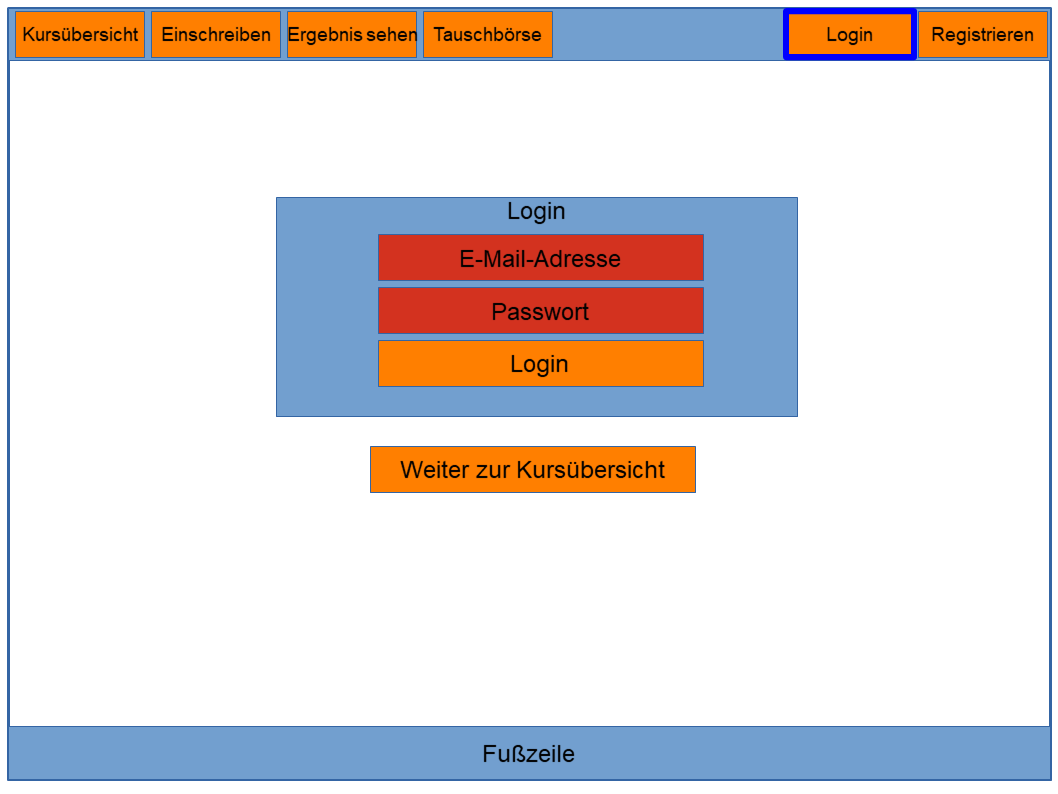
\includegraphics[width=\textwidth]{./implementation/images/MockUpsFrontend/frontendLogin.png}
	            \end{subfigure}
	            \begin{subfigure}{\textwidth}
	                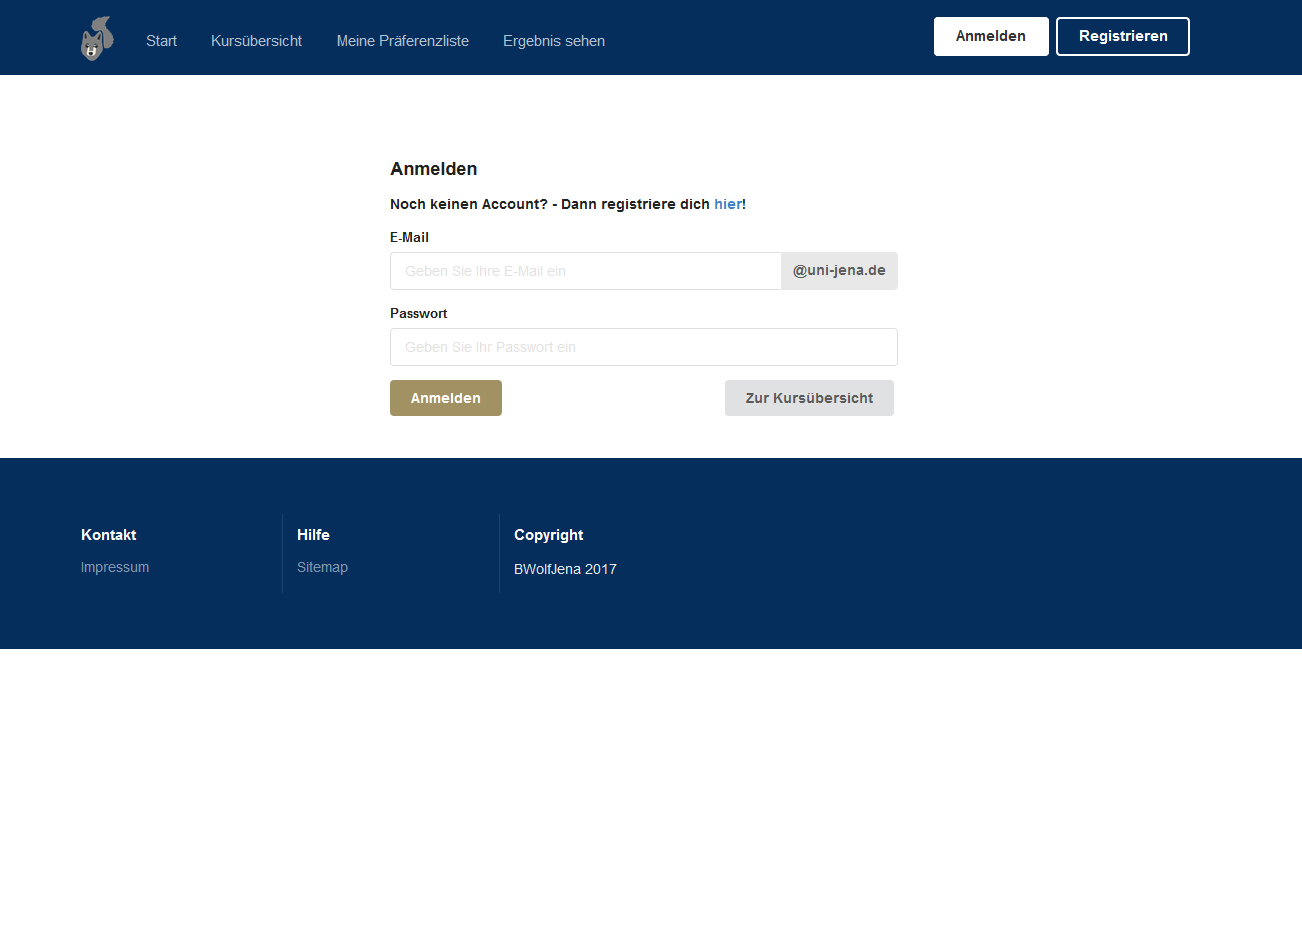
\includegraphics[trim={5cm 0 5cm 0}, clip, width=\textwidth]{./implementation/images/login.png}
	            \end{subfigure}
	            \caption{Gegenüberstellung von Entwurf der Login-Oberfläche und Umsetzung }
	            \label{fig:comparisonLogin}
	       \end{figure}
	    
    
        In Abbildung \ref{fig:comparisonLogin} sind der Entwurf für die Login-Oberfläche und die Umsetzung selbiger gegenüber gestellt.
        Es fällt auf, dass die grobe Struktur der Seite bis auf kleine Änderungen mit dem Entwurf übereinstimmt.
        Unterschiede lassen sich vor allem in der Kopfzeile erkennen.
        So wurde der Reiter \textit{Start} hinzugefügt.
        Anders als zuvor angedacht, fiel die Entscheidung für eine Startseite, in der das Empiriepraktikum kurz vorgestellt wird.
        Des Weiteren wurde der Reiter \textit{Einschreiben} aus Gründen der Verständlichkeit in \textit{Meine Präferenzliste} umbenannt.
        Die Seite erfüllt jedoch die selbe Funktion.
	        \begin{figure}[p]
	            \centering
	            \begin{subfigure}{\textwidth}
	                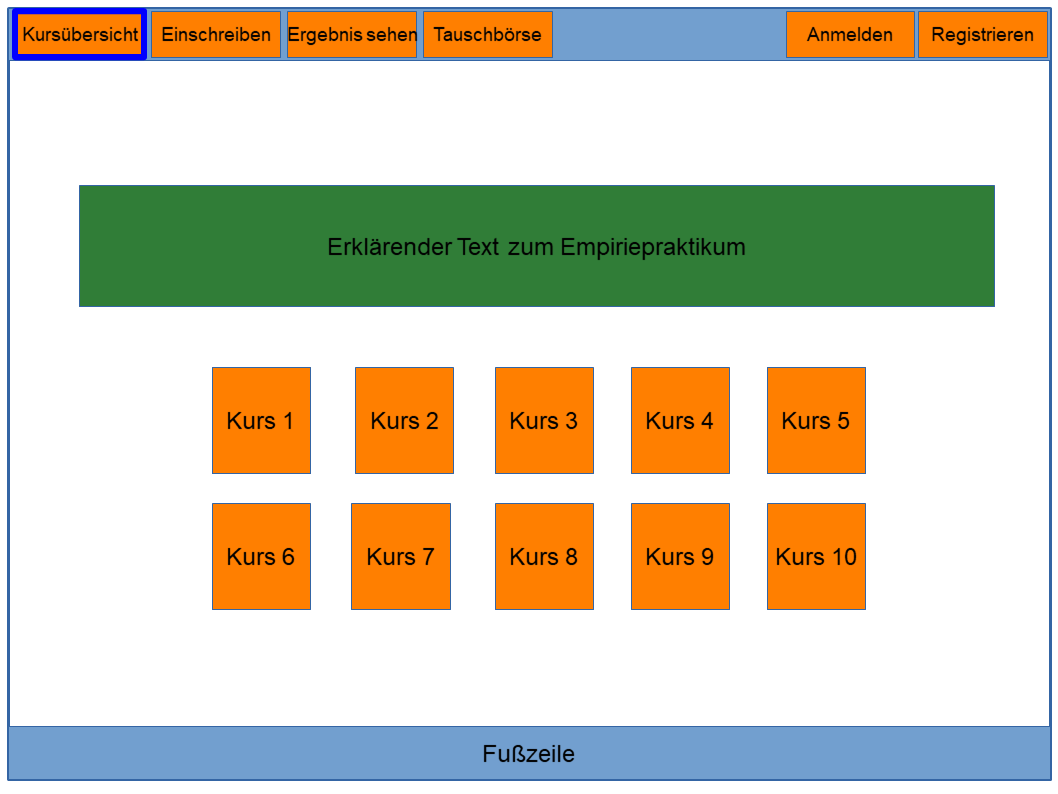
\includegraphics[width=1.0\textwidth]{./implementation/images/MockUpsFrontend/frontendCourses.png}
	            \end{subfigure}
	            \begin{subfigure}{\textwidth}
	                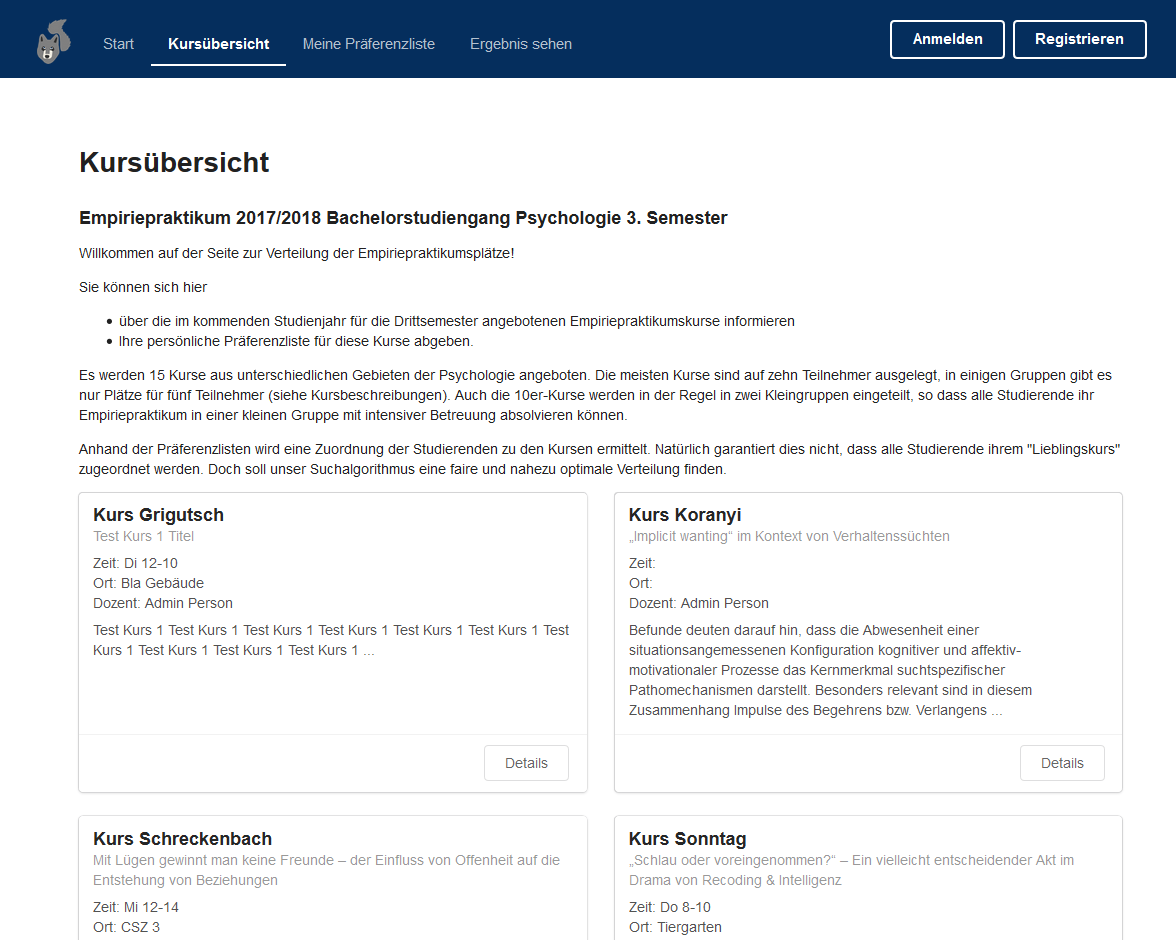
\includegraphics[trim={12cm 5cm 12cm 0},clip,width=1.0\textwidth]{./implementation/images/courses.png}
	            \end{subfigure}
	            \caption{Gegenüberstellung von Entwurf der Kursübersicht und Umsetzung}
	            \label{fig:comparisonCourses}
	        \end{figure}
	    
    
        Abbildung \ref{fig:comparisonCourses} zeigt Entwurf und Umsetzung der Kursübersicht.
        Die Struktur des Entwurfs wurde direkt umgesetzt.
        Wie in Kapitel \ref{chapter:requirements} beschrieben, ist es, wie in Abbildung \ref{fig:comparisonCourses} zu sehen ist, möglich auch ohne eine Anmeldung auf die Kursübersicht zuzugreifen.
        Es ist anzumerken, dass die Fußleiste auch in der Kursübersicht \ref{fig:comparisonCourses} den Abschluss der Seite bildet und lediglich durch die Menge an Kursen nicht zu sehen ist.
        \afterpage{
	        \begin{figure}[p]
	            \centering
	            \begin{subfigure}{0.8\textwidth}
	                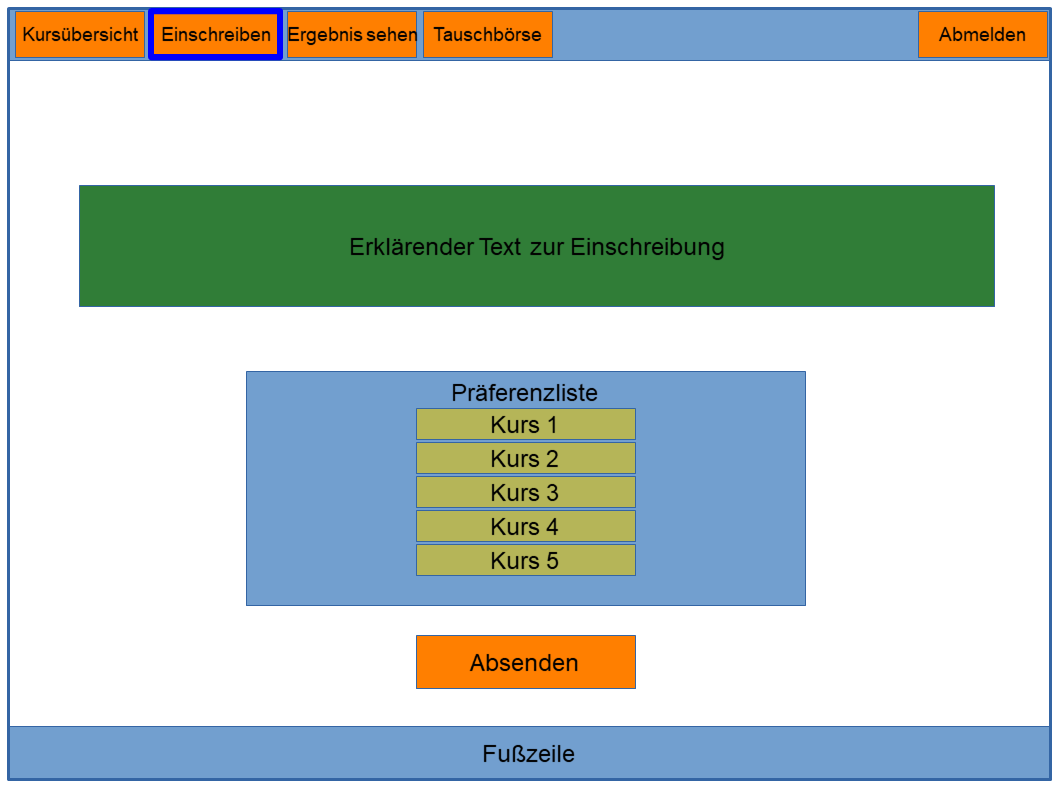
\includegraphics[width=1.0\textwidth]{./implementation/images/MockUpsFrontend/frontendPreferences.png}
	            \end{subfigure}
	            \begin{subfigure}{\textwidth}
	                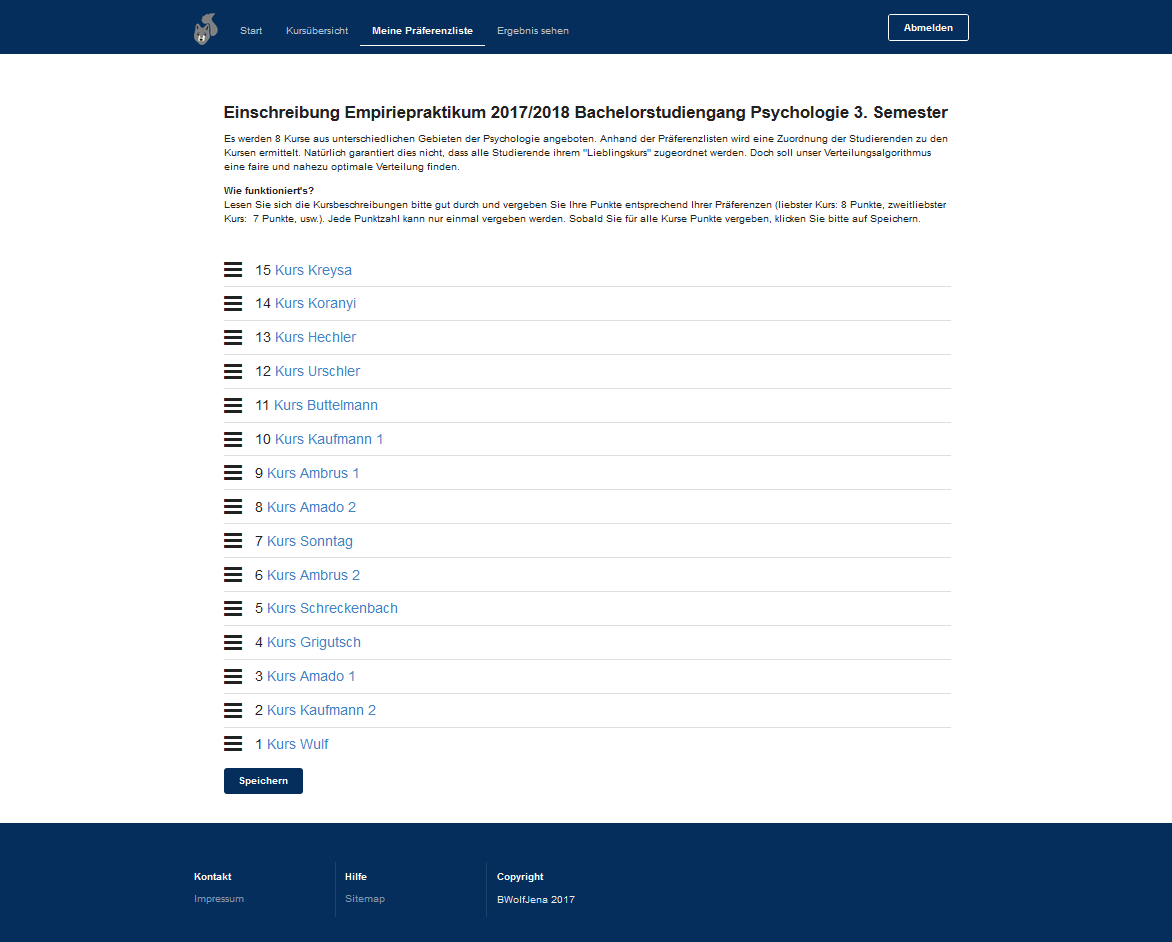
\includegraphics[trim={15cm 0cm 15cm 0},clip,width=\textwidth]{./implementation/images/preferences.png}
	            \end{subfigure}
	            \caption{Gegenüberstellung von Entwurf der Einschreibungs-Oberfläche und Umsetzung}
	            \label{fig:comparisonPrefenrences}
	        \end{figure}
	    }
    
        Die Oberfläche zum Erstellen der Präferenzliste wurde ebenfalls wie angedacht umgesetzt.
        Mithilfe von Drag\&Drop könne die verschiedenen Kurse in die gewünschte Reihenfolge gebracht werden.
        Der Knopf \textit{Absenden} wurde in \textit{Speichern} umbenannt.
        Dadurch soll mehr Klarheit darüber geschaffen werden, dass die Präferenzliste bis zum Ablauf der Frist jederzeit verändert werden kann.\\
        
        Es ist zu erwähnen, dass das gesamte Frontend auch auf mobilen Geräten unterstützt wird.
        Die Ansichten für Kursübersicht und auch die Wahl der Präferenzliste werden entsprechend der Größe des Bildschirms angepasst, sodass die Benutzerfreundlichkeit erhalten bleibt.\\
        
        Die Tauschbörse wurde nicht implementiert.
        Grund hierfür ist zum einen die zeitliche Beschränkung des Projekts, wodurch einige optionale Funktionalitäten nicht umgesetzt werden konnten.
        Zum anderen sind bei einem weiteren Gespräch nach dem Erstellen der Anforderungen Zweifel an der Notwendigkeit solch einer Tauschbörse aufgetreten.
        Eine weitere Funktion, die nicht im Frontend umgesetzt werden konnte, war die in Kapitel \ref{chapter:design} geplante Erweiterbarkeit auf andere Module.
        So kann ein Benutzer im Frontend nicht mehrere Präferenzlisten parallel verwalten.\\
        
        Im Frontend wurde jedoch auch eine zusätzliche Funktionalität implementiert.
        So wurde ein Archiv umgesetzt, in dem die Kurse vergangener Empiriepraktika einsehbar sind.
    
    \section{Backend}
        Auch im Backend ist die Struktur der Entwürfe weitestgehend übernommen worden.
        \afterpage{
	        \begin{figure}[p]
	            \centering
	            \begin{subfigure}{\textwidth}
	                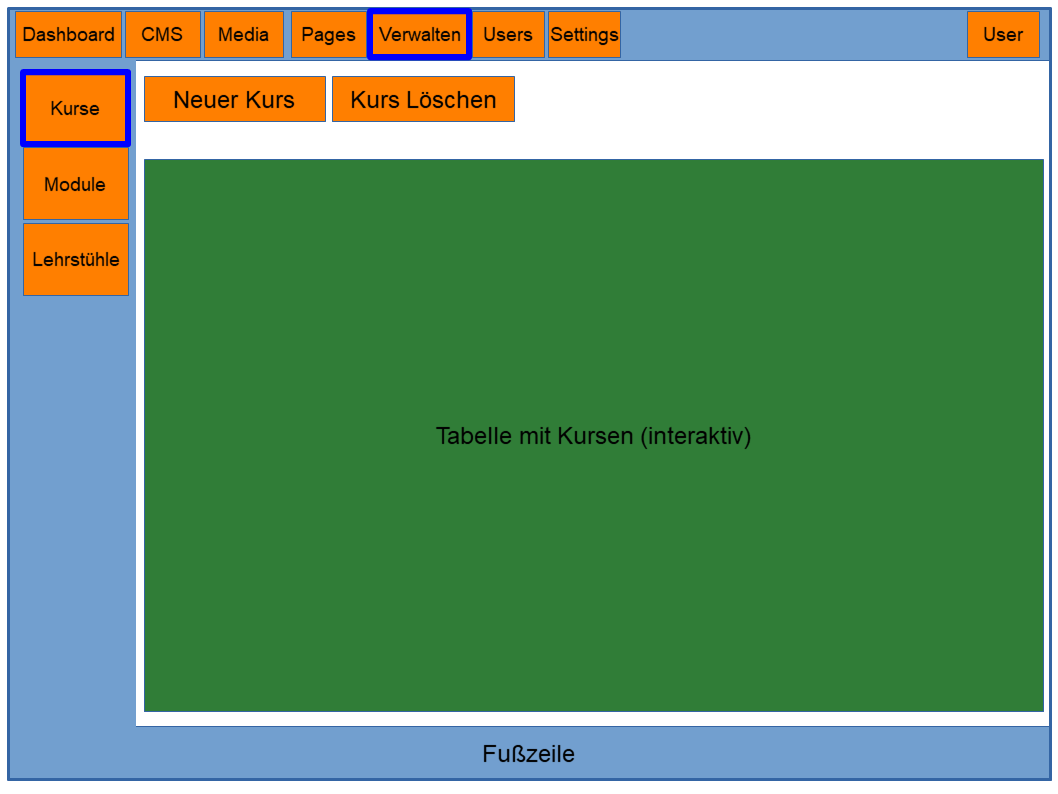
\includegraphics[width=1.0\textwidth]{./implementation/images/MockUpsBackend/backendManageCourses.png}
	            \end{subfigure}
	            \begin{subfigure}{\textwidth}
	                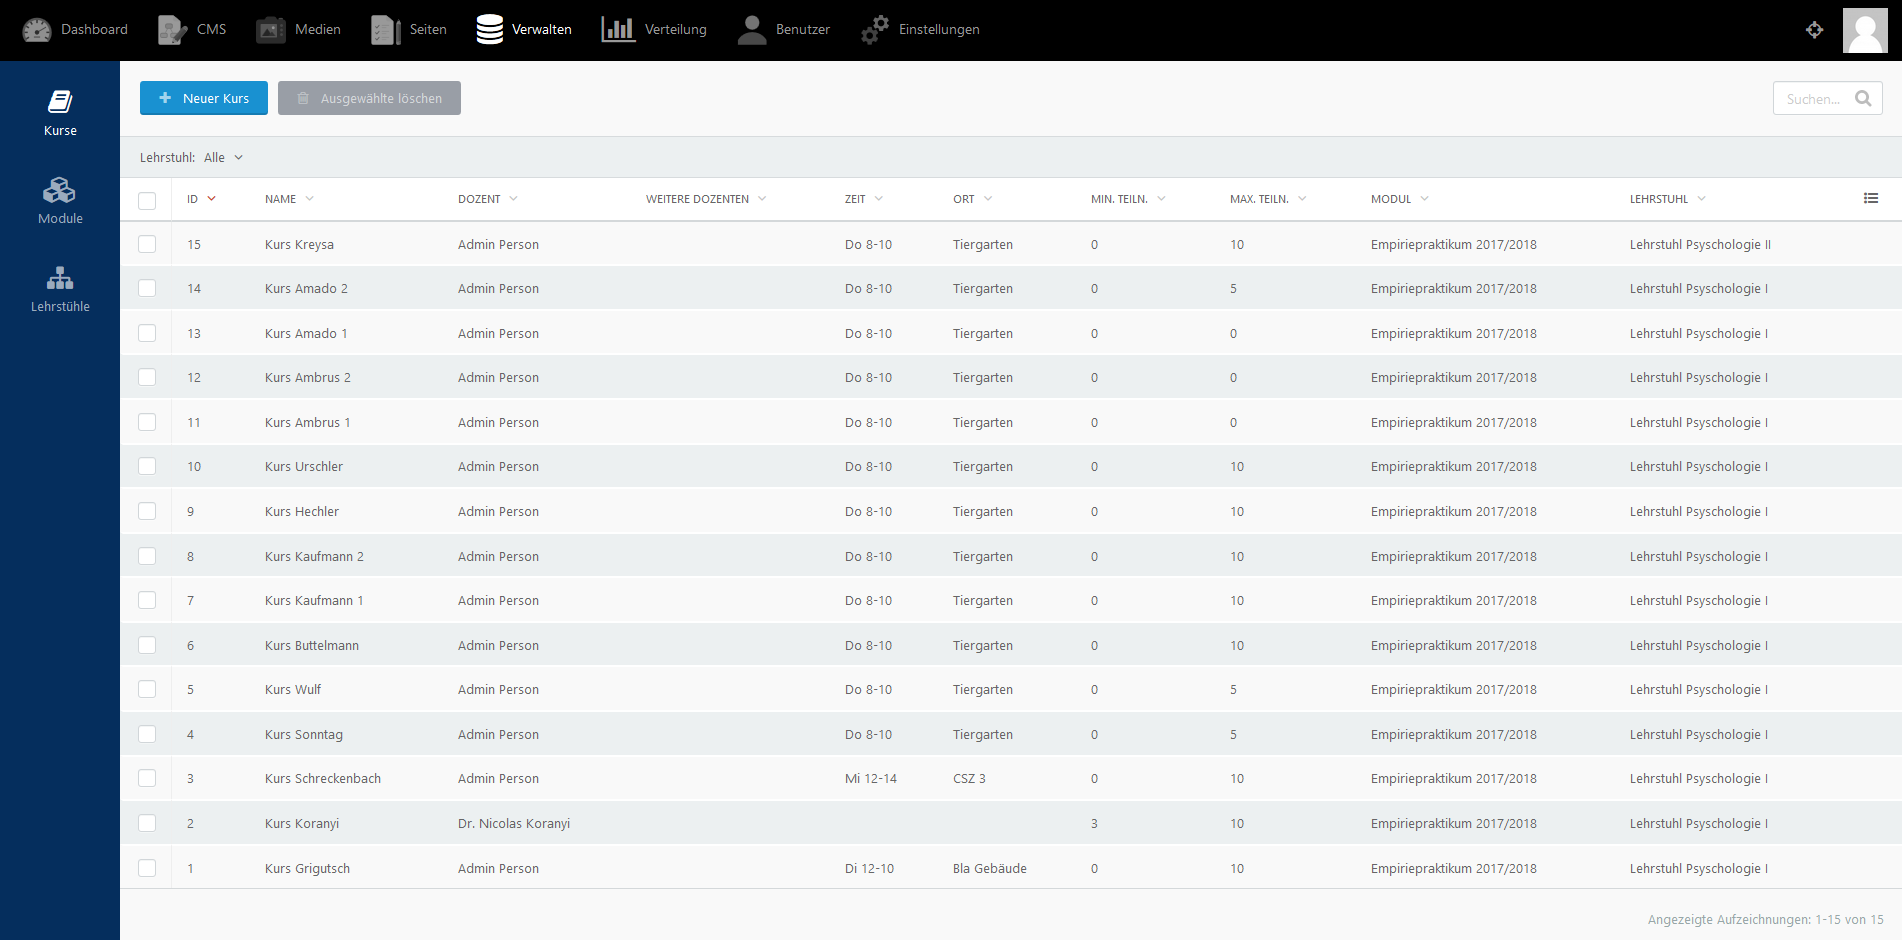
\includegraphics[width=1.0\textwidth]{./implementation/images/manageCourses.png}
	            \end{subfigure}
	            \caption{Gegenüberstellung von Entwurf der Kursverwaltung und Umsetzung}
	            \label{fig:comparisonManageCourses}
	        \end{figure}
	    }
        
        Abbildung \ref{fig:comparisonManageCourses} zeigt Entwurf und Umsetzung der Kursverwaltung.
        Die Struktur aus Kopf- und Seitenleiste wurde übernommen.
        Die Fußzeile wurde jedoch entfernt.
        Es fällt außerdem auf, dass die Kopfzeile mehr Reiter umfasst, als zunächst geplant.
        Das zum Erstellen des Backend verwendete Framework \textit{October CMS} stellt einige vordefinierte Seiten zur Verfügung. Da von Beginn an geplant war für die entsprechenden Funktionen ein CMS zu verwenden wurden dafür keine Mockups erstellt.
        Darunter fällt das \textit{Dashboard}, in dem zum Start des Backends einige wichtige Informationen angezeigt werden.
        Unter dem Reiter \textit{Seiten} können weitere Seiten für das Frontend erstellt und die vorhanden Seiten bearbeitet werden.
        Der Reiter \textit{Einstellungen} ist ebenfalls von \textit{October CMS} bereitgestellt und erlaubt das Ändern und Verwalten verschiedenster Optionen.
        Für dieses Projekt relevant sind vor allem die Einstellungen bezüglich der automatisch versendeten E-Mails, sowie das Verwalten der Backendbenutzer.
        Anders als im Entwurf vorgesehen, werden nicht alle Benutzer über den Reiter \textit{Benutzer} verwaltet, sondern nur die Frontendnutzer.
        Diese Änderung ist durch \textit{October CMS} bedingt.
        
        \begin{figure}[p]
            \centering
            \begin{subfigure}{\textwidth}
                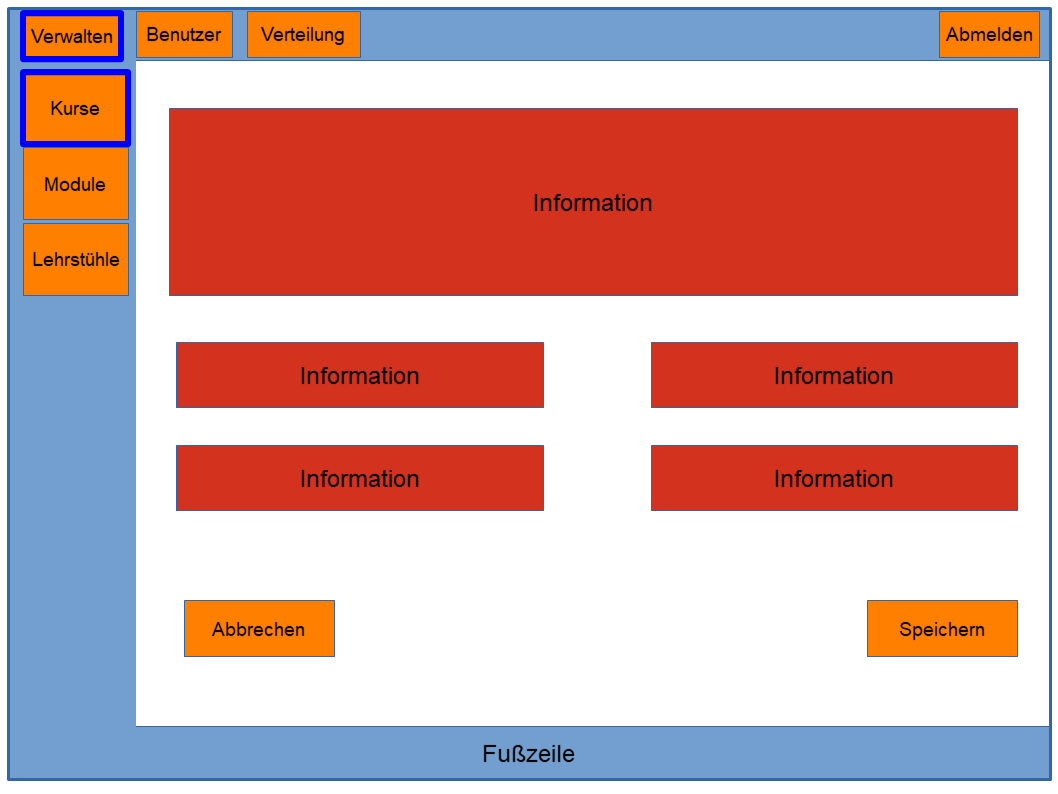
\includegraphics[width=1.0\textwidth]{./implementation/images/MockUpsBackend/backendEdit.png}
            \end{subfigure}
            \begin{subfigure}{\textwidth}
                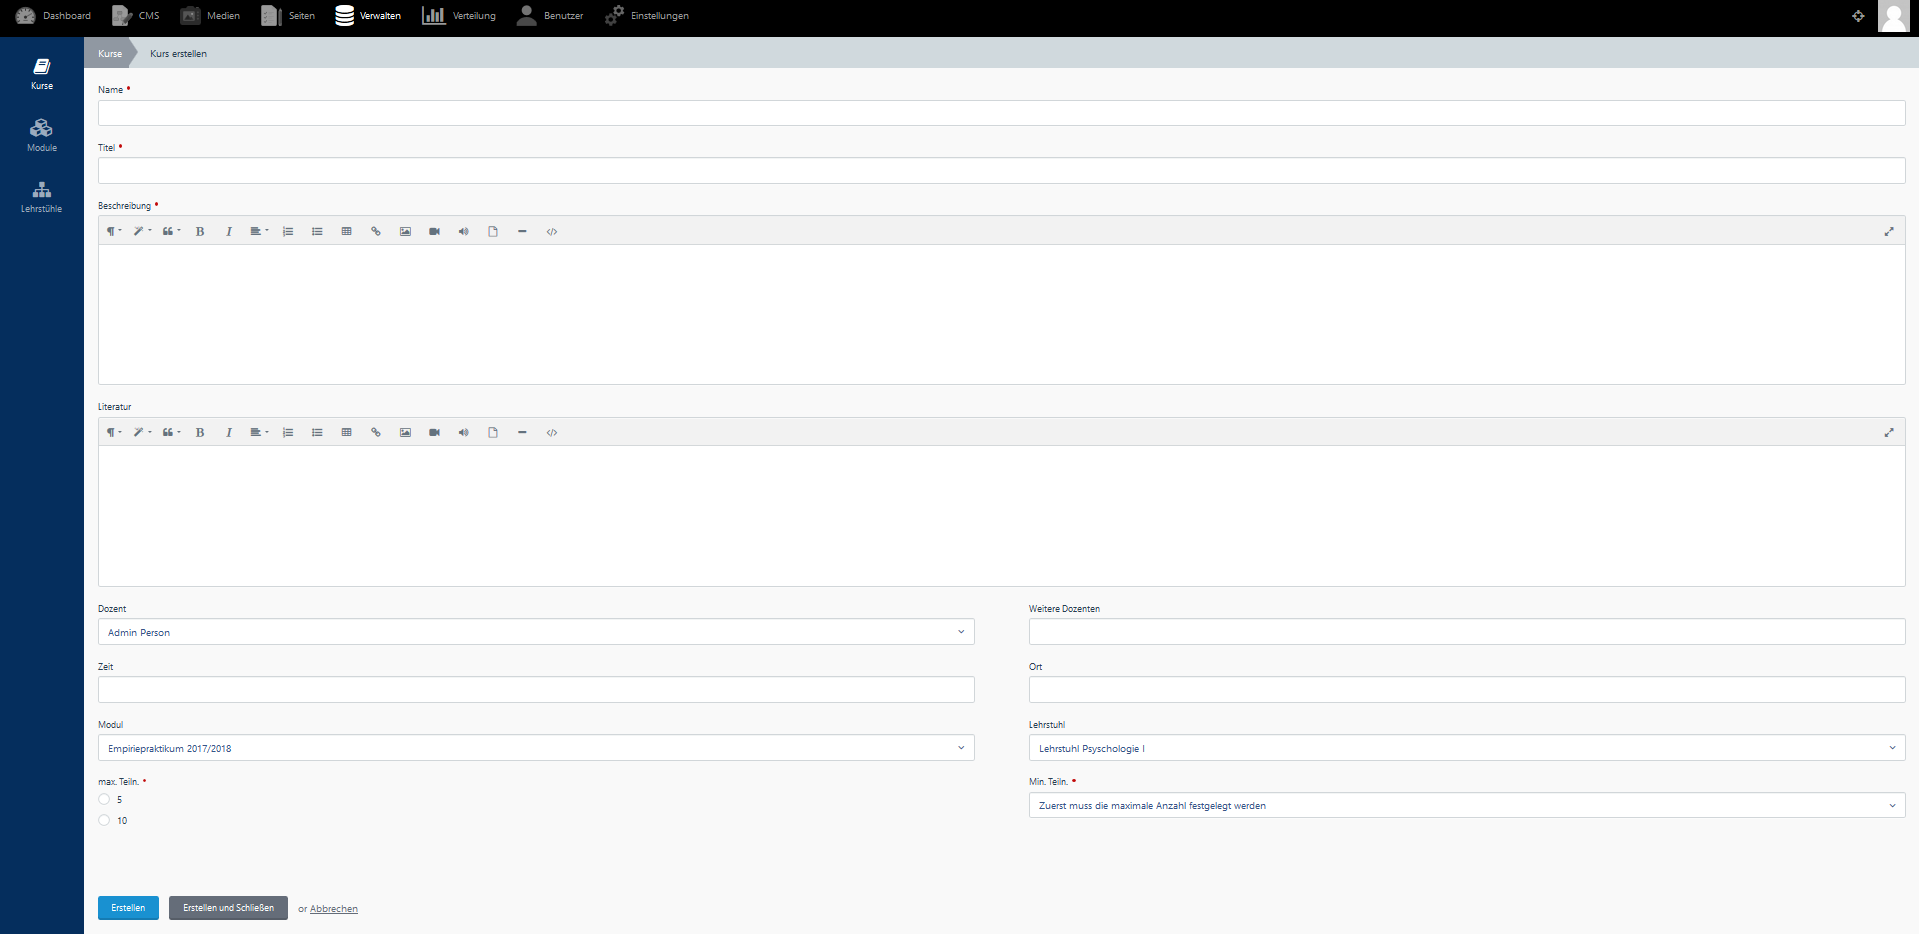
\includegraphics[width=1.0\textwidth]{./implementation/images/edit.png}
            \end{subfigure}
            \caption{Gegenüberstellung von Entwurf der Kurserstellung und Umsetzung}
            \label{fig:comparisonEdit}
        \end{figure}
    
        Das Erstellen und Bearbeiten von Kursen, Lehrstühlen, Benutzern, usw. ist, wie in Abbildung \ref{fig:comparisonEdit} zu sehen, wie im Entwurf umgesetzt.
        Verschiedene Eingabefelder mit \textit{Richtext}-Bearbeitung und Auswahlfelder werden wie vorgesehen zur Verfügung gestellt.
    
        \begin{figure}[p]
            \centering
            \begin{subfigure}{0.9\textwidth}
                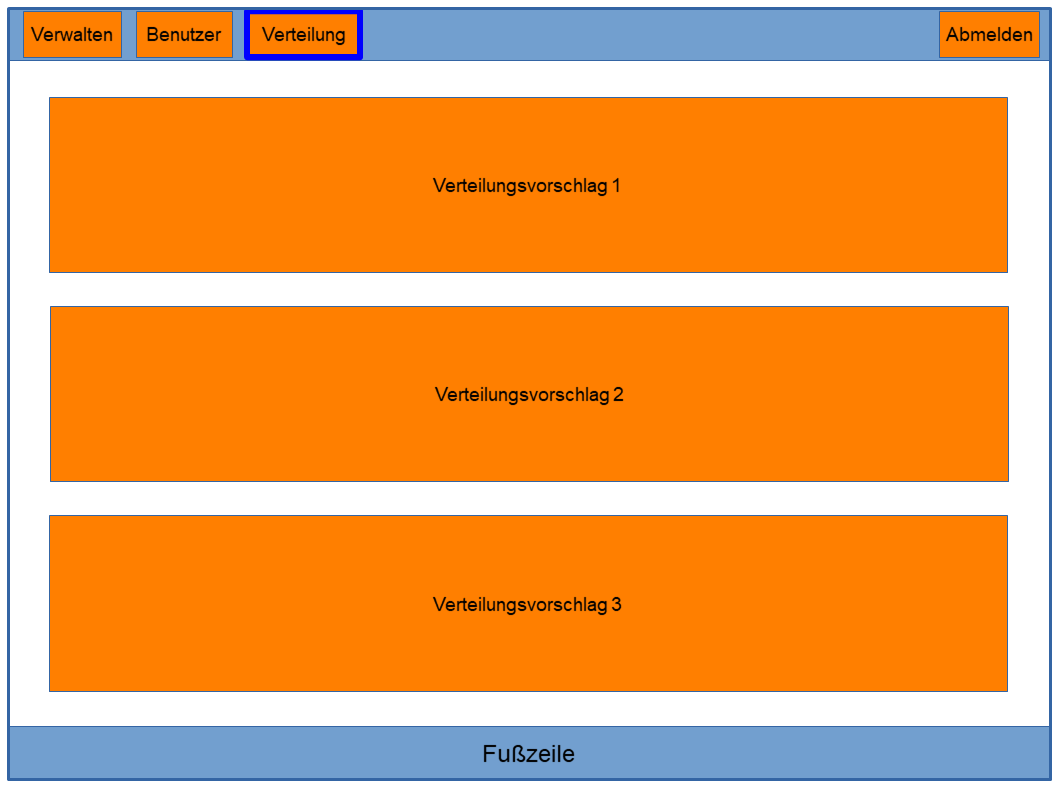
\includegraphics[width=1.0\textwidth]{./implementation/images/MockUpsBackend/backendDistribution.png}
            \end{subfigure}
            \begin{subfigure}{\textwidth}
                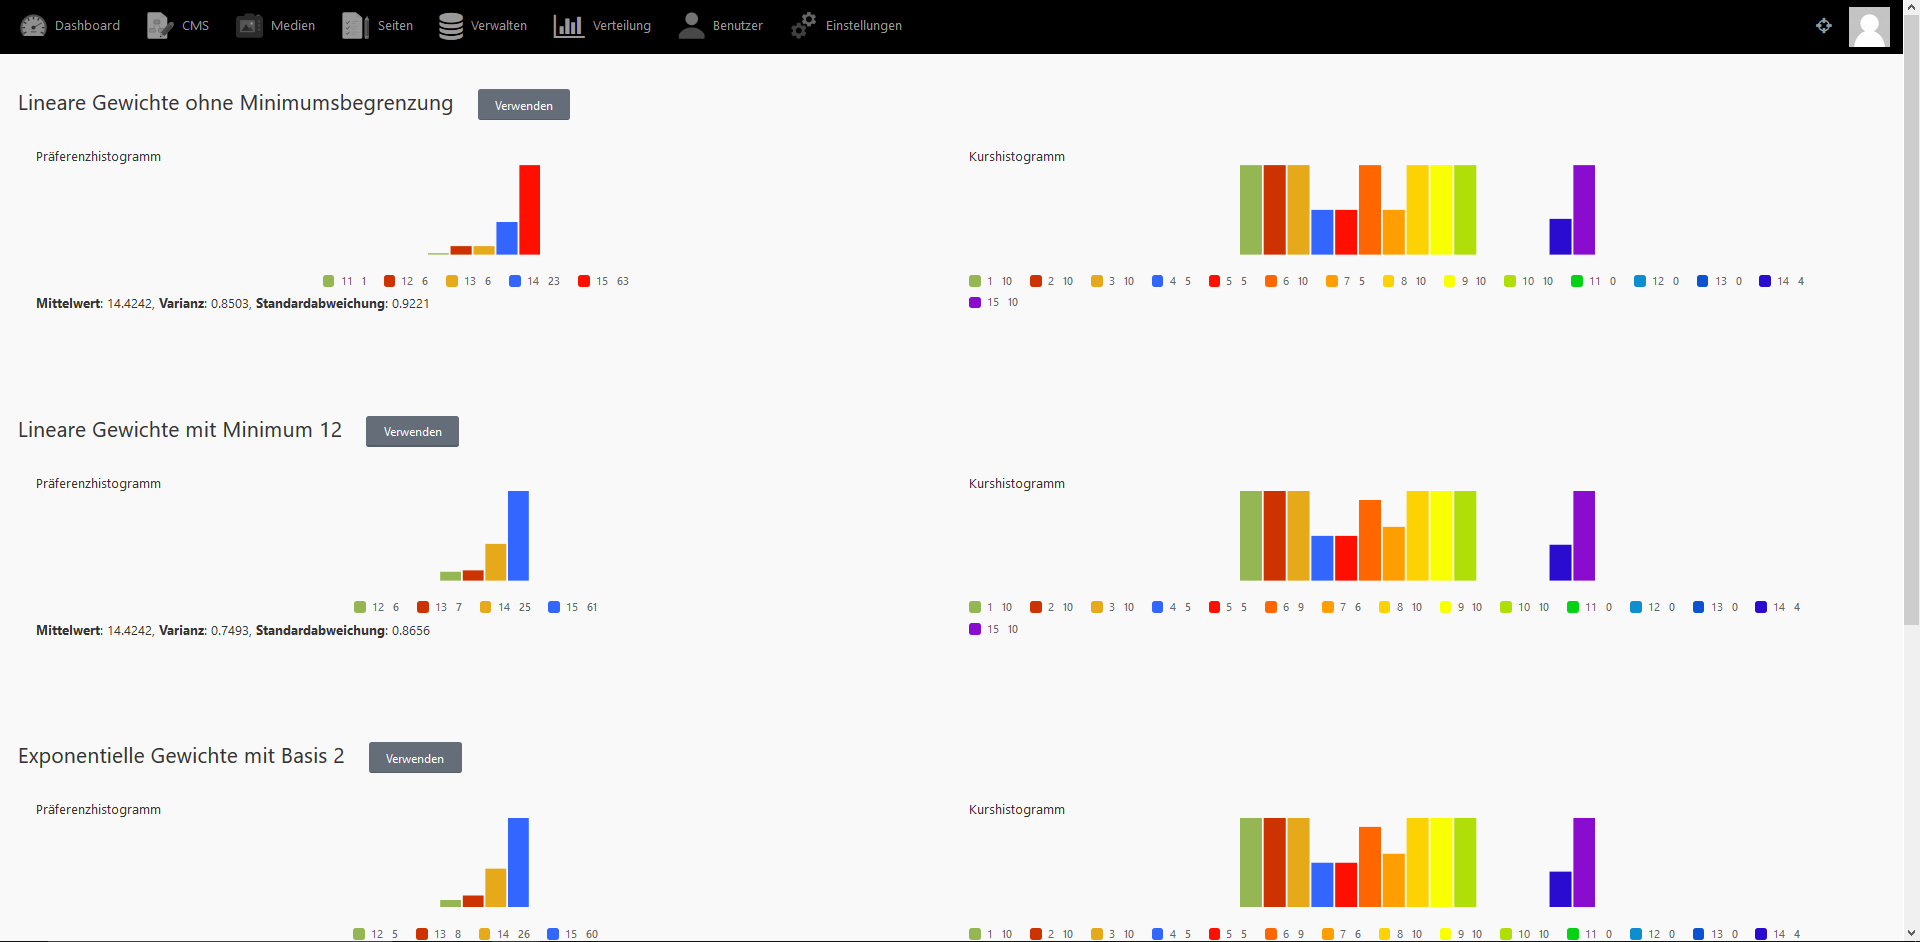
\includegraphics[width=1.0\textwidth]{./implementation/images/distribution.png}
            \end{subfigure}
            \caption{Gegenüberstellung von Entwurf der Anzeige der Verteilungsvorschläge und Umsetzung}
            \label{fig:comparisonDistribution}
        \end{figure}
    
        Auch der Entwurf der Verteilungsansicht wurde umgesetzt.
        In Abbildung \ref{fig:comparisonDistribution} sind wieder Mockup und Resultat gegenübergestellt.
		\pagebreak

    \section{Algorithmus}
	Da lange unbekannt war, ob die für den Algorithmus verwendete Software \textit{lp\_solve}\footnote{\href{http://lpsolve.sourceforge.net/5.5/index.htm}{http://lpsolve.sourceforge.net/5.5/index.htm}} auf dem Server laufen würde, wird der Algorithmus auf einem externen Server ausgeführt. 
    Dazu wurde ein HTTP-Service in \textit{Node.js} implementiert, der eine Liste mit Kursteilnehmerbegrenzungen, die Präferenzlisten (nur IDs), sowie die Parameter für den Algorithmus (minPref, weights) entgegennimmt und mit der Lösung des in Kapitel \ref{chapter:algorithm} beschriebenen Optimierungsproblems antwortet.	
    Da es kein Budget für das Projekt gab, wird der Server dauerhaft kostenlos bei \textit{Heroku} \footnote{\href{https://www.heroku.com/home}{https://www.heroku.com/home}} gehostet. 
    Nach 30 Minuten Inaktivität geht er dabei in den Ruhezustand wodurch die nächste Anfrage ein paar Sekunden langsamer beantwortet wird. 
    Falls \textit{Heroku} diesen Service einstellen sollte, kann der Algorithmus auch lokal ausgeführt werden. 
    Eine Anleitung wie die lokale Umgebung installiert wird befindet sich in der Anwenderdokumentation. 
    Die Daten müssen dann mit Hilfe eines \textit{MySQL} Clients vom Server der Universität exportiert und lokal importiert werden. 
    Zum Exportieren und Importieren von Daten befindet sich ebenfalls ein Abschnitt in der Anwenderdokumentation. 
    
    
    
    
    
